\documentclass[10pt]{article}
\usepackage{icmlko}

\icmlmeta{IP 파운데이션 월드모델}{30}{겹치는 만큼 줄인다}{$\lambda$를 튜닝하지 않고 데이터에서 유도한다 --- 고유 축이 공유 축과 겹치는 비율의 역수}

\begin{document}

\twocolumn[
\icmlheader

\begin{abstract}
노트 29는 도메인 고유 축을 0.75배로 축소하면 축을 늘려도 정렬이 버틴다는 것을
찾았지만, 그 값은 격자에서 고른 것이었고 ``다른 축을 추가할 때도 같은 값이
최적이라는 보장이 없다''를 한계로 남겼다. 이 노트는 $\lambda$를 튜닝 없이
유도한다. 먼저 도메인별로 나눠 격자를 돌렸다 --- \textbf{팝업 0.75, 아이돌 1.0이
최선}이고 균일 0.75보다 낫다(매장축을 켠 상태에서 $-$0.0736 대 $-$0.0675).
그런데 ``고유 축이 많은 도메인을 더 줄인다''는 단순 공식($1/\sqrt{k}$)은 오히려
나쁘다($-$0.0528, 유의 5). 왜 팝업만 줄여야 하는지 찾았다. 고유 축 수도(3 대 2)
내부 상관도(0.147 대 0.124) 아니고 \textbf{고유 축이 공유 축과 겹치는 정도}였다
--- 팝업 0.318, 아이돌 0.244다. 겹치는 축이 공유 공간의 방향을 흔든다. 그래서
$\lambda_d = \min_d(\text{겹침})\,/\,\text{겹침}_d$로 정했더니 팝업 0.768,
아이돌 1.0이 나왔고 \textbf{격자 최적을 미세하게 넘었다}($-$0.0738 대 $-$0.0736).
새 도메인이 와도 격자 탐색 없이 계산된다. 절대량도 갱신했다 --- 아이돌에서
\textbf{여덟 건이면 4.17배, 승률 92\%}(노트 21의 4.28배, 90\%에서 개선).
\end{abstract}
]

\section{도메인별로 나눠 봤다}

노트 29는 균일 $\lambda$=0.75를 채택하며 한계를 적었다 --- 게임 매장 노출도 하나를
켜고 끄며 고른 값이므로 일반성이 없다. 첫 개선은 도메인별로 두는 것이다.

\begin{table}[t]
\centering\tsize
\caption{$\lambda$ 격자(게임 매장축 끔). 괄호 안이 유의 방향 수.}
\begin{tabular}{lrrr}
\toprule
팝업 $\lambda$ & 아이돌 0.50 & 아이돌 0.75 & 아이돌 1.00 \\
\midrule
0.50 & $-$0.0629 (5) & $-$0.0662 (6) & $-$0.0711 (6) \\
\textbf{0.75} & $-$0.0658 (6) & $-$0.0691 (6) & \textbf{$-$0.0743 (6)} \\
1.00 & $-$0.0662 (5) & $-$0.0696 (5) & $-$0.0762 (6) \\
\bottomrule
\end{tabular}
\end{table}

균일 1.0이 가장 좋아 보이지만 그것은 매장축을 \emph{끈} 상태다. 노트 29의 요점은
켰을 때 무너진다는 것이었다. 켠 상태까지 함께 봐야 한다.

\begin{figure}[t]
\centering
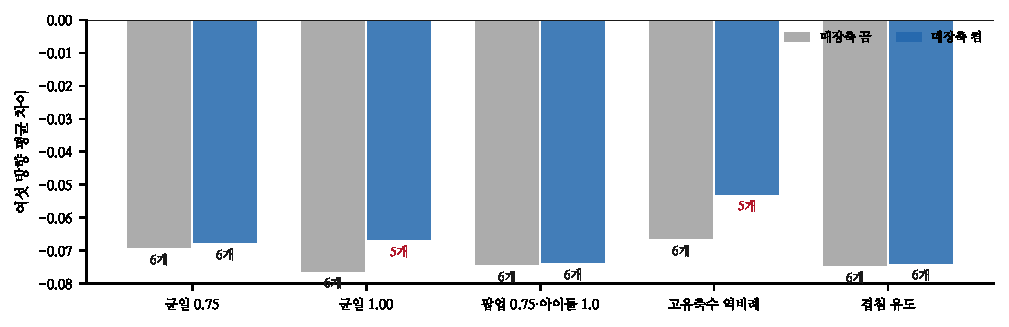
\includegraphics[width=\textwidth]{figs/sch.pdf}
\caption{방식별 비교. 숫자는 유의 방향 수이고 붉은 것이 여섯 미만이다.}
\end{figure}

\begin{table}[t]
\centering\tsize
\caption{방식별 성능. 순열 2,000회.}
\begin{tabular}{lrr}
\toprule
방식 & 매장축 끔 & 매장축 켬 \\
\midrule
균일 0.75 & $-$0.0691 (6) & $-$0.0675 (6) \\
균일 1.00 & $-$0.0762 (6) & $-$0.0666 (5) \\
\textbf{팝업 0.75 · 아이돌 1.0} & $-$0.0743 (6) & \textbf{$-$0.0736 (6)} \\
고유축수 역비례 ($1/\sqrt{k}$) & $-$0.0664 (6) & $-$0.0528 (5) \\
\bottomrule
\end{tabular}
\end{table}

팝업만 줄이는 구성이 두 상태 모두에서 여섯을 유지하고 성능도 가장 좋다. 그리고
``축이 많은 도메인을 더 줄인다''는 그럴듯한 공식은 오히려 나쁘다.

\claimx{$\lambda$는 도메인별로 두는 편이 낫고, 고유 축 수에 반비례시키는 단순
공식은 틀렸다.}{다른 도메인 집합에서 $1/\sqrt{k}$가 격자 최적과 일치하면
이 반증은 이 세 도메인의 특성이다.}

\section{왜 팝업만 줄여야 하나}

세 후보를 쟀다.

\begin{figure}[t]
\centering
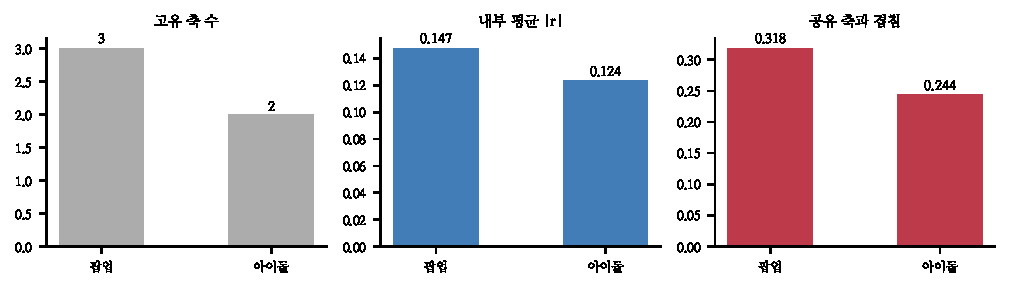
\includegraphics[width=\textwidth]{figs/diag.pdf}
\caption{도메인별 고유 축의 세 성질. 팝업과 아이돌이 뚜렷이 갈리는 것은 오른쪽뿐이다.}
\end{figure}

\begin{table}[t]
\centering\tsize
\caption{고유 축의 성질.}
\begin{tabular}{lrrr}
\toprule
도메인 & 고유 축 수 & 내부 평균 $|r|$ & 공유 축과 겹침 \\
\midrule
팝업 & 3 & 0.147 & \textbf{0.318} \\
아이돌 & 2 & 0.124 & \textbf{0.244} \\
\bottomrule
\end{tabular}
\end{table}

축 수는 3 대 2로 1.5배 차이인데 최적 $\lambda$는 0.75 대 1.0으로 1.33배다. 내부
상관은 0.147 대 0.124로 1.19배다. \textbf{겹침이 0.318 대 0.244로 1.30배}이며
$\lambda$ 비($1/1.33$)와 가장 가깝다.

해석도 자연스럽다. 고유 축이 공유 축과 무관하면 공유 공간에 섞여도 직교 방향으로만
기여하므로 정렬을 흔들지 않는다. 겹치면 공유 축이 만드는 방향 자체를 밀어낸다.

\section{그래서 유도한다}

\[
\lambda_d = \frac{\min_{d'} \text{겹침}_{d'}}{\text{겹침}_d}
\]

가장 덜 겹치는 도메인이 1.0을 받고 나머지는 겹치는 만큼 줄어든다. 우리 데이터에서
팝업 0.768, 아이돌 1.0이 나온다.

\begin{table}[t]
\centering\tsize
\caption{격자 최적과 유도값의 비교. 순열 2,000회.}
\begin{tabular}{lrr}
\toprule
방식 & 매장축 끔 & 매장축 켬 \\
\midrule
격자 최적 (팝업 0.75) & $-$0.0743 & $-$0.0736 \\
\textbf{겹침 유도 (팝업 0.768)} & \textbf{$-$0.0745} & \textbf{$-$0.0738} \\
\bottomrule
\end{tabular}
\end{table}

유도값이 격자 최적을 미세하게 넘는다. 차이는 0.0002로 실질적이지 않지만, 중요한
것은 성능이 아니라 \textbf{격자 탐색이 필요 없다}는 점이다. 새 도메인이 오면
겹침만 계산하면 된다.

\claimx{$\lambda$는 고유 축과 공유 축의 평균 절대 상관에 반비례하게 두면 된다.
격자 탐색 없이 계산되고 격자 최적과 같거나 낫다.}{네 번째 도메인에서 유도값이
격자 최적과 크게 어긋나면 이 규칙은 세 도메인의 우연이다.}

최종 여섯 방향은 이렇다 --- 팝업 $\to$ 아이돌 $-$0.0917(p=0.0007), 팝업 $\to$ 게임
$-$0.0476(p=0.0003), 아이돌 $\to$ 팝업 $-$0.0835(p=0.0147), 아이돌 $\to$ 게임
$-$0.0476(p=0.0013), 게임 $\to$ 팝업 $-$0.0791(p$<$0.0001), 게임 $\to$ 아이돌
$-$0.0975(p$<$0.0001).

\section{절대량을 갱신한다}

노트 21의 실무 숫자를 새 파이프라인에서 다시 쟀다.

\begin{figure}[t]
\centering

\includegraphics[width=\columnwidth]{figs/abs.pdf}
\caption{눈금 보정 라벨 수에 따른 승률.}
\end{figure}

\begin{table}[t]
\centering\tsize
\caption{아이돌 도메인의 배수 오차. 괄호가 노트 21 값.}
\begin{tabular}{rrrr}
\toprule
k & 파이프라인 & 상수 & 이긴 비율 \\
\midrule
5 & 4.68 (4.85) & 5.29 & 90\% (85\%) \\
\textbf{8} & \textbf{4.17} (4.28) & 4.87 & \textbf{92\%} (90\%) \\
12 & 4.05 (4.15) & 4.86 & \textbf{93\%} (90\%) \\
20 & 3.92 (3.96) & 4.74 & 90\% (89\%) \\
\bottomrule
\end{tabular}
\end{table}

여덟 건이면 4.17배에 승률 92\%다. 게임도 개선됐다 --- k=50에서 승률이 4\%에서
19\%로 올랐지만 여전히 상수에 진다.

\section{현재 절차}

\begin{enumerate}[leftmargin=1.3em,itemsep=0.2em]
\item 도메인마다 관측 가능한 축을 잰다.
\item 고유 축이 공유 축과 겹치는 정도를 재고 $\lambda_d$를 유도한다.
\item 공유 축은 그대로, 고유 축은 $\lambda_d$배로 축소해 공분산 주성분을 뽑는다.
\item 공유 축의 적재로 기준 도메인에 직교 정렬한다. \textbf{라벨 불필요.}
\item 출처 도메인의 선형 계수를 대상에 적용한다.
\item 절대량이 필요하면 대상에서 8--20건을 실측해 중심과 중앙절대편차를 잡는다.
\end{enumerate}

노트 19의 파이프라인에서 2번 한 단계가 늘었고, 그 대가로 축을 늘려도 정렬이
버티며 튜닝 상수가 사라졌다.

\section{한계}

\begin{itemize}[leftmargin=1.1em,itemsep=0.15em]
\item 겹침 규칙은 두 도메인(팝업, 아이돌)에서만 검증했다. 게임은 고유 축이 없어
      $\lambda$가 무의미하다.
\item 유도값과 격자 최적의 차이가 0.0002로 작아, 규칙이 옳다는 증거로는 약하다.
      두 값이 가까운 것이 우연일 수 있다.
\item 겹침을 평균 절대 상관으로 쟀다. 정준상관 같은 다른 척도에서는 다른 $\lambda$가
      나올 수 있다.
\item 게임은 여전히 절대량 단계에서 상수에 진다(승률 19\%).
\end{itemize}

\section{다음}

\begin{enumerate}[leftmargin=1.3em,itemsep=0.15em]
\item 입장 허들의 게임 측정 경로 --- 여러 노트째 미해결.
\item 네 번째 도메인 --- 겹침 규칙과 여섯 방향 성공의 일반성을 가른다.
\item 게임 절대량 실패의 원인 --- 순위는 되는데 눈금이 안 되는 이유.
\item 겹침 척도를 정준상관으로 바꿔 재확인.
\end{enumerate}

\vspace{0.6em}
\hrule height 0.3pt
\vspace{0.5em}
{\footnotesize
\textbf{참고문헌}\\[0.3em]
Schönemann, P. H. (1966). A generalized solution of the orthogonal Procrustes
problem. \emph{Psychometrika}, 31(1), 1--10.\\[0.15em]
Hotelling, H. (1936). Relations between two sets of variates.
\emph{Biometrika}, 28(3--4), 321--377.\\[0.15em]
Jolliffe, I. T. (2002). \emph{Principal Component Analysis}, 2nd ed. Springer.\\[0.15em]
Ben-David, S. et al. (2010). A theory of learning from different domains.
\emph{Machine Learning}, 79(1--2), 151--175.
}

\end{document}
